\documentclass[journal]{IEEEtran}
\usepackage[utf8]{inputenc}
\usepackage[T1]{fontenc}
\usepackage{amsmath,amssymb}
\usepackage{booktabs}
\usepackage{array}
\usepackage{url}
\usepackage[hidelinks]{hyperref}
\usepackage{cite}
\usepackage{float}
\usepackage{pgfplots}
\pgfplotsset{compat=1.18}
\usepgfplotslibrary{groupplots}
\definecolor{barA}{RGB}{70,90,120}
\definecolor{barB}{RGB}{190,120,70}
\definecolor{barC}{RGB}{120,140,110}

\newcommand{\sB}{S_B}

\begin{document}

\title{Do Language Models Follow a Fixed Doctrine?\\A Decomposition Benchmark for Real-Time Strategy Macro Decisions}

\author{{\large Ruo-Ze Liu}\\[0.6ex]
Nanjing University, Nanjing, China\\[0.3ex]
\texttt{liuruoze@163.com}}

\markboth{Technical Report, November 2026}{Decomposition Benchmark for RTS Macro Decisions}

\maketitle

\begin{abstract}
Real-time strategy games are a standard testbed for sequential decision making, but a deployed
commander does not only need to win: it must execute a doctrine its author can state in rules.
We ask whether open-weight language models can apply such a doctrine, and find that the answer
depends far more on how the question is asked than on how large the model is. We build a frozen
120-item benchmark from a Protoss zealot-rush doctrine expressed as five independent yes/no
decisions, with labels derived from the rules themselves rather than from game outcomes. Three
audits, including a second independent implementation of the rules, verify every item. Across
six models from 7B to 32B parameters, asking for all five bits in one answer collapses every
model onto a single repeated vector: the best scores 0.237 on a scale where doing nothing scores
0.158. Asking five separate yes/no questions transforms the result. The same 32B model rises to
0.925, and to 0.967 when the state is rendered as JSON, over 240 items with a 95\% interval of
[0.950, 0.981]. Two counter-intuitive results accompany this: prompt refinements tuned on a
weaker model \emph{reduce} the stronger model's score, and self-consistency over three samples
changes nothing because the errors are systematic rather than noisy.
\end{abstract}

\begin{IEEEkeywords}
large language models, real-time strategy, StarCraft II, instruction following, benchmark,
prompt decomposition, evaluation methodology
\end{IEEEkeywords}

\section{Introduction}

StarCraft II has served for a decade as a demanding test of autonomous agents~\cite{vinyals2019}.
The celebrated results in that line of work are reinforcement learning systems trained to win,
and their competence is measured in league points. A different question arises when a language
model is placed in the commander's seat of an existing, hand-written strategy. There the
requirement is not to discover a policy but to \emph{execute a stated one}: given a snapshot of
the game, decide which of several known actions are warranted right now, according to rules a
human author has written down.

This distinction matters for practice. Practitioners who attach a language model to a game bot
usually do so because they want the bot to follow a doctrine they can read, audit and modify,
not because they want a second learner competing with the first. Whether current open-weight
models can do this, and at what size, is an empirical question that, to our knowledge, has not
been posed in a controlled way.

We pose it on a concrete doctrine: a Protoss zealot rush, reduced by its author to five
independent decisions---build a pylon, train a probe, build a gateway, train a zealot, attack.
Each decision has an explicit threshold. Because the decisions are independent (a probe can
build while a gateway trains), the natural output is a five-bit vector rather than a single
choice among alternatives, and the natural scoring is per-item and partially credit-bearing.

Our contributions are:
\begin{itemize}
\item a frozen, audited 120-item benchmark with a parallel 120-item set for checking
generalisation, in which labels follow from the doctrine's rules and not from win/loss;
\item a scoring rule calibrated against trivial baselines, so that a model which never acts
scores 0.158 rather than the 0.517 that naive partial credit would award;
\item an empirical result with a clear shape: decomposition dominates scale, and prompt
refinements that help a small model harm a large one;
\item an error analysis locating the residual failures in a single rule, and a latency
measurement against a 30-second deployment gate.
\end{itemize}

\section{Related Work}

\textbf{Agents in StarCraft.} AlphaStar reached grandmaster level with a combination of
imitation learning, league self-play and a carefully engineered interface~\cite{vinyals2019}.
The SC2 learning environment~\cite{vinyals2017} and PySC2 made the game accessible to
researchers. These systems learn policies; we instead test whether a pretrained model can apply
a policy that is given to it in words.

\textbf{Language models as agents.} ReAct interleaves reasoning with acting~\cite{yao2023}, and
Voyager builds open-ended Minecraft skills from a language model's prior~\cite{wang2023voyager}.
Both report successes with large models and few-shot prompting. Our result suggests a boundary
condition: on a task requiring several simultaneous threshold checks, models below roughly 32B
parameters do not merely degrade, they collapse to a constant output.

\textbf{Instruction following and prompt sensitivity.} Chain-of-thought prompting improves
multi-step reasoning at sufficient scale~\cite{wei2022}, and self-consistency improves it
further by voting over samples~\cite{wang2023sc}. Prompt formatting alone can move benchmark
scores substantially~\cite{sclar2024}, which motivates the multi-prompt reporting advocated by
Mizrahi et al.~\cite{mizrahi2024}. We find the same sensitivity, and in a direction worth
flagging: a prompt variant selected on a 14B model degraded a 32B model by ten points.

\textbf{Evaluation methodology.} HELM~\cite{liang2023} and BIG-bench~\cite{srivastava2023}
established multi-task, standardised evaluation; MT-Bench and its judge analysis
\cite{zheng2023} address open-ended generation. Our setting is narrower and fully automatic:
labels are computed, not judged, so no judge model enters the loop.

\section{Benchmark Design}

\subsection{The doctrine as five decisions}

The author's zealot-rush doctrine is stated as five rules over seven observable quantities:
elapsed time $t$, supply used and cap, minerals, probe count, zealot count, gateway count and
pylon count. Supply cap is $15 \times \text{nexus} + 8 \times \text{pylons}$, capped at 200.
Table~\ref{tab:rules} gives the rules verbatim in translation. The rules are evaluated
independently; the only positional dependency is that a gateway cannot be placed without a
pylon's power field.

\begin{table}[t]
\centering
\caption{The five decisions, as given to the model. ``Gap'' is cap minus used supply.}
\label{tab:rules}
\footnotesize
\begin{tabular}{@{}p{0.9cm}p{6.3cm}@{}}
\toprule
Bit & Rule \\
\midrule
1 & Pylon: none exist, or (gap $\le 9$ and cap $<200$) \\
2 & Probe: probes $\le 14$ and gap $\ge 1$ \\
3 & Gateway: gateways $<3$ and at least one pylon \\
4 & Zealot: zealots $<24$, minerals $\ge 100$, probes $\ge 10$, gateways $\ge 1$, gap $\ge 2$ \\
5 & Attack: zealots $\ge 8$ \\
\bottomrule
\end{tabular}
\end{table}

\subsection{Why multiple labels}

A single-choice framing would force the model to pick one action per tick, which the game does
not require: probe production, unit production and construction proceed in parallel. We
therefore elicit a five-bit vector and score each bit independently, which also yields a
diagnostic per rule rather than a single opaque number.

\subsection{Scoring}

Let $w$ be the Hamming distance between the predicted and the true five-bit vector. A response
scores $1.0$ if $w=0$, $0.5$ if $w=1$, and $0$ otherwise; the item score is the mean over
items. This choice is not cosmetic. If any partial answer earns half credit, a model that
answers \texttt{00000} to everything scores $0.517$ on our set, because on almost every item at
least one bit of zeros is correct, and the usable range of the metric collapses to
$[0.5,1]$. Under the rule above, the same degenerate strategy scores $0.158$; a single
heuristic (``attack when zealots $\ge 8$'') scores $0.221$; the doctrine itself scores $1.000$.

\subsection{Item construction and auditing}

Items comprise 31 boundary cases and 89 random states. Boundary items are built in pairs that
differ in exactly one quantity, straddling a threshold (14/15 probes, 2/3 gateways, 7/8
zealots, 9/10 gap, 99/100 minerals, and so on); the four sparsest thresholds carry four items
each. Random states sample supply, units and buildings jointly.

Three constraints make a state physically possible, and each was added after an audit found
violations: capacity follows the pylon count; unit count never exceeds supply; and the build is
feasible in time and in minerals (at most $12 + t/12$ probes, $1 + t/45$ gateways, $(t/27)$
times the gateway count in zealots, and total spend within $1.25\times$ estimated mining).

Labels are computed by \texttt{doctrine.py}. A second implementation, written independently
from the protocol text and sharing no code, recomputes all 600 bits; the two agree on every
item. Further checks confirm the rendered prompt contains each state value, that no prompt
leaks the answer, that no two items share a state, and that the eight boundary pairs each flip
exactly the bit they are named for. A parallel set of 120 items is generated with a different
seed under identical rules and passes the same checks; it is used only to test generalisation.

\section{Experimental Setup}

\textbf{Models.} Qwen2.5-Instruct at 7B, 14B and 32B; Qwen3-8B and Qwen3-32B; GLM-4-9B-chat.
All are open-weight and served locally.

\textbf{Serving.} A single-process OpenAI-compatible server per model, bfloat16, greedy
decoding (temperature 0), 512-token cap for whole-task answers. Models larger than one 24\,GB
card are sharded across GPUs by \texttt{accelerate}. Qwen3 is run with thinking disabled via
its template flag.

\textbf{Protocols.} \emph{Whole-task}: one request per item, system prompt contains all five
rules, answer is five bits. \emph{Decomposed}: five requests per item, each system prompt
contains only the rule being asked, answer is yes or no; the five answers are concatenated.

\textbf{Parsing.} Any thinking block is stripped, non-binary characters removed, and the
remaining digits read; for yes/no replies the first explicit affirmation or negation is taken.

\section{Results}

\begin{table}[t]
\centering
\caption{Score $\sB$ by model and protocol on the frozen set (120 items). ``Split'' is five
yes/no requests per item with the rule text verbatim. Bold marks the best configuration.}
\label{tab:main}
\footnotesize
\begin{tabular}{@{}lccc@{}}
\toprule
Model & Whole-task & Split & Split, tuned \\
\midrule
Qwen2.5-7B   & 0.167 & 0.292 & --- \\
Qwen2.5-14B  & 0.208 & 0.558 & 0.646 \\
Qwen2.5-32B  & 0.237 & 0.925 & \textbf{0.967} \\
Qwen3-8B     & 0.200 & 0.308 & --- \\
Qwen3-32B    & ---   & 0.479 & --- \\
GLM-4-9B     & 0.113 & 0.050 & --- \\
\midrule
\multicolumn{4}{@{}l}{\emph{Baselines}: attack-if-8 0.221; do nothing 0.158} \\
\bottomrule
\end{tabular}
\end{table}


\begin{figure}[t]
\centering
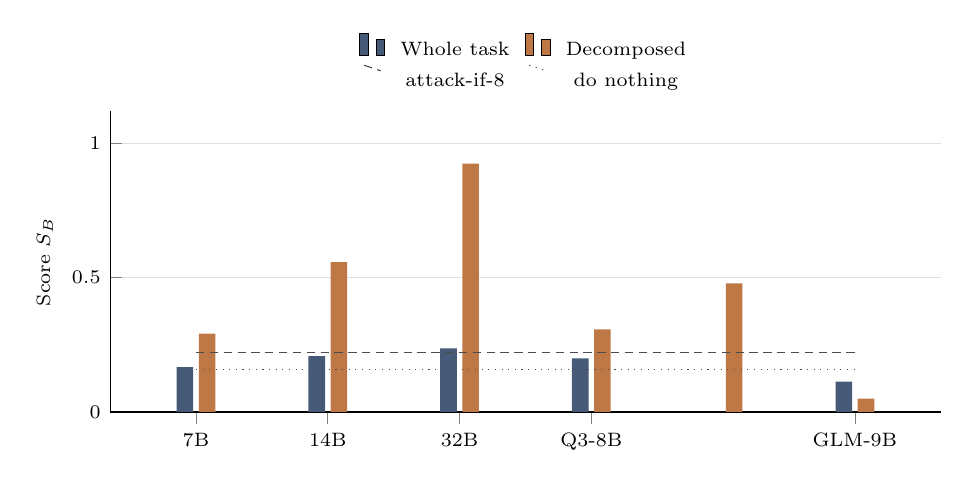
\begin{tikzpicture}
\begin{axis}[
  ybar, bar width=6pt,
  width=\columnwidth, height=5.4cm,
  ymin=0, ymax=1.12,
  ylabel={Score $S_B$},
  symbolic x coords={7B,14B,32B,Q3-8B,Q3-32B,GLM-9B},
  xtick=data,
  x tick label style={font=\scriptsize},
  y tick label style={font=\scriptsize},
  ylabel style={font=\scriptsize},
  legend style={font=\scriptsize, at={(0.5,1.03)}, anchor=south,
                legend columns=2, draw=none, column sep=0.8ex},
  enlarge x limits=0.13,
  axis lines*=left,
  ymajorgrids, grid style={black!12},
]
\addplot[fill=barA, draw=none] coordinates
  {(7B,0.167) (14B,0.208) (32B,0.237) (Q3-8B,0.200) (GLM-9B,0.113)};
\addplot[fill=barB, draw=none] coordinates
  {(7B,0.292) (14B,0.558) (32B,0.925) (Q3-8B,0.308) (Q3-32B,0.479) (GLM-9B,0.050)};
\addplot[black!70, densely dashed, sharp plot, update limits=false] coordinates
  {(7B,0.221) (GLM-9B,0.221)};
\addplot[black!70, dotted, sharp plot, update limits=false] coordinates
  {(7B,0.158) (GLM-9B,0.158)};
\legend{Whole task, Decomposed, attack-if-8, do nothing}
\end{axis}
\end{tikzpicture}
\caption{Score by model under the two protocols, with the two trivial baselines drawn across.
The whole-task bars sit near the baselines for every model; decomposition separates them by
size. Qwen3-32B was run decomposed only.}
\label{fig:scores}
\end{figure}

\subsection{Whole-task answers collapse}

Table~\ref{tab:main} shows that no model exceeds 0.237 when asked for five bits at once, and the
spread between the 7B and the 32B is 0.07---far short of the 0.63 that separates them under
decomposition. Inspection of the outputs explains why: each model repeats one vector
almost regardless of input. The 7B answers \texttt{10110} on 73 of 120 items, the 14B
\texttt{00010} on 75, GLM \texttt{01110} on 52. Replacing every answer with the model's modal
vector reproduces its score to within 0.017 for the 14B and 0.046 for the 7B; for GLM the
substitution \emph{improves} the score, meaning its variation is worse than a constant.
Two of the five bits are answered below chance by the 7B (42\% on pylon, 46\% on gateway), which
is the signature of a fixed vector rather than of partial competence: the failure is not a
missing threshold but the absence of any item-specific computation.

\subsection{Decomposition changes the result}

Asking the same five questions separately lifts every model that can follow a single rule
(Table~\ref{tab:main}). The 32B moves from 0.237 to 0.925, the 14B from 0.208 to 0.558, the 7B
from 0.167 to 0.292. Two do not improve: Qwen3-32B answers \emph{yes} to almost everything
(per-bit accuracies of 62\% and 69\% where the positive rate is 44\% and 41\%), and GLM-4-9B
does the same, scoring 0.050. Both appear to treat the yes/no form as an invitation to agree.

\subsection{Scale matters only within the right form}

Holding the protocol fixed, the Qwen2.5 family orders cleanly: 0.292, 0.558, 0.925 at 7B, 14B
and 32B. Across protocols the ordering breaks: a 32B asked for five bits (0.237) is worse than
a 14B asked one rule at a time (0.558). Task form and model size are not interchangeable
levers; form dominates.


\begin{figure*}[t]
\centering
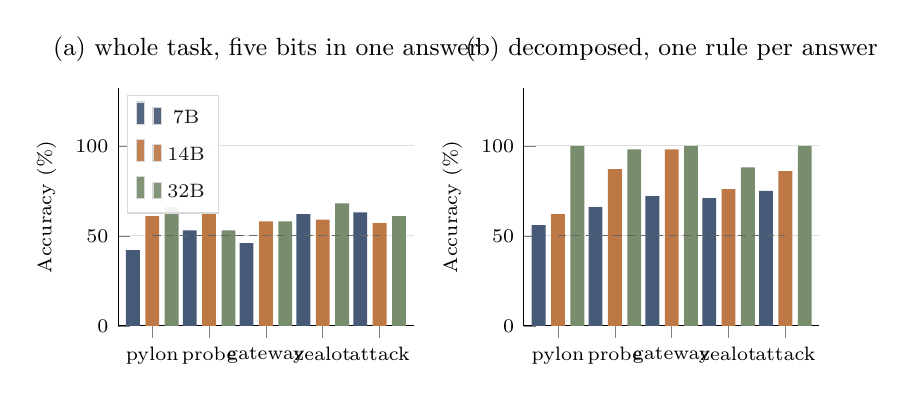
\begin{tikzpicture}
\begin{groupplot}[
  group style={group size=2 by 1, horizontal sep=1.4cm},
  width=0.44\textwidth, height=4.6cm,
  ymin=0, ymax=132,
  ylabel={Accuracy (\%)},
  symbolic x coords={pylon,probe,gateway,zealot,attack},
  xtick=data,
  x tick label style={font=\scriptsize},
  y tick label style={font=\scriptsize},
  ylabel style={font=\scriptsize},
  legend style={font=\scriptsize, at={(0.03,0.97)}, anchor=north west,
                legend columns=1, fill=white, fill opacity=0.92,
                draw=black!15, row sep=0.5ex},
  axis lines*=left, ymajorgrids, grid style={black!12},
  enlarge x limits=0.15,
]
\nextgroupplot[ybar, bar width=5pt, title={(a) whole task, five bits in one answer}, title style={font=\small}]
\addplot[fill=barA, draw=none] coordinates
  {(pylon,42) (probe,53) (gateway,46) (zealot,62) (attack,63)};
\addplot[fill=barB, draw=none] coordinates
  {(pylon,61) (probe,62) (gateway,58) (zealot,59) (attack,57)};
\addplot[fill=barC, draw=none] coordinates
  {(pylon,66) (probe,53) (gateway,58) (zealot,68) (attack,61)};
\draw[densely dashed, black!60] (axis cs:pylon,50) -- (axis cs:attack,50);
\legend{7B,14B,32B}
\nextgroupplot[ybar, bar width=5pt, title={(b) decomposed, one rule per answer}, title style={font=\small}]
\addplot[fill=barA, draw=none] coordinates
  {(pylon,56) (probe,66) (gateway,72) (zealot,71) (attack,75)};
\addplot[fill=barB, draw=none] coordinates
  {(pylon,62) (probe,87) (gateway,98) (zealot,76) (attack,86)};
\addplot[fill=barC, draw=none] coordinates
  { (pylon,100) (probe,98) (gateway,100) (zealot,88) (attack,100)};
\draw[densely dashed, black!60] (axis cs:pylon,50) -- (axis cs:attack,50);
\end{groupplot}
\end{tikzpicture}
\caption{Per-bit accuracy for the three Qwen2.5 sizes. In (a) every model stays within sixteen
points of chance on every rule, and the 7B falls below it on two. In (b) the same models
separate: the 32B is exact on three rules, and its one weak rule---zealot production---is the
same rule that carries almost all of its residual error in Table~\ref{tab:errors}. Dashed line
marks 50\%.}
\label{fig:perbit}
\end{figure*}

\subsection{Prompt variants, and a transfer failure}

\begin{table}[t]
\centering
\caption{Prompt variants on the 32B model, same items and protocol. All rows are decomposed
answers.}
\label{tab:variants}
\footnotesize
\begin{tabular}{@{}lc@{}}
\toprule
Variant & $\sB$ \\
\midrule
Rule text verbatim, state as JSON & \textbf{0.967} \\
Rule text verbatim, state as prose & 0.925 \\
Emphasise ``gateway must already exist'' & 0.917 \\
Reframe as capability question & 0.900 \\
Enumerated five-line checklist & 0.892 \\
Rewrite rules in plainer Chinese & 0.846 \\
Verbatim rules + three worked examples per rule & 0.850 \\
Plainer rules + examples & 0.829 \\
\bottomrule
\end{tabular}
\end{table}

Table~\ref{tab:variants} varies the prompt while holding the model and items fixed. The
verbatim rule text wins. Every refinement we introduced---plainer wording, worked examples, an
emphatic restatement of the gateway precondition, reframing the question as ``can a zealot be
trained right now'', an enumerated checklist---lowers the score.

The same refinements had been developed on the 14B, where they \emph{raised} the score from
0.558 to 0.646. Applied to the 32B, the identical prompt dropped it from 0.925 to 0.829. A
prompt selected on a weaker model is not merely suboptimal for a stronger one; it is actively
harmful. We attribute this to the examples: the 14B needs them to locate the threshold, while
the 32B reads the threshold from the rule and is then anchored to the numbers in the examples.

Rendering the state as a JSON object rather than prose lifts the 32B by four points. The
information is identical; the format is not.

\subsection{Where the residual errors are}

\begin{table}[t]
\centering
\caption{Error structure of the best configuration on the frozen set (17 of 120 items not
exact). False positives dominate, and most involve a missing gateway.}
\label{tab:errors}
\footnotesize
\begin{tabular}{@{}lccc@{}}
\toprule
Quantity & False pos. & False neg. & Of the false pos., no gateway \\
\midrule
Zealot (bit 4) & 15 & 0 & 10 \\
Probe (bit 2)  & 0  & 3 & --- \\
\bottomrule
\end{tabular}
\end{table}

Fifteen of seventeen imperfect items miss the zealot bit, and all fifteen are false positives:
the model recommends training when the rule says not to (Table~\ref{tab:errors}). Ten of those
states have no gateway at all. The model appears to reason that a gateway is about to be built,
so the unit may be queued---a defensible inference that the literal rule forbids. The remaining
three items err in the opposite direction on the probe bit: the model declines to train probes
in states where the rule permits it. Every other bit is answered correctly on every item.

Emphasising the precondition did not help (0.917). Reframing the question as a capability
(``can a zealot be trained right now'') cut false positives from 15 to 6 but introduced 15
false negatives, for a worse total; the model then treats a marginal gateway count as a reason
to abstain. An enumerated five-line checklist scored 0.892. The failure is not a missing
threshold but an interaction: the model applies ``zealots $<24$'' and ``minerals $\ge 100$''
correctly in isolation and overrides ``gateways $\ge 1$'' when the other two hold.

\subsection{Self-consistency and latency}

Three samples at temperature 0.7 with majority voting leave the 14B's score unchanged at 0.675
(versus 0.675 single-sample, exact match 50.0\% versus 49.2\%). The errors are systematic, so
resampling does not decorrelate them. Greedy decoding is deterministic: two runs of the best
configuration agree on every item.

Latency per item, five requests, single server: 0.39\,s for the 7B, 1.88\,s for the 32B
(p95 2.31\,s). The deployment gate allows 30\,s per decision with eight concurrent games, which
requires 1.33 requests per second; one 32B instance sustains about 2.6. Qwen3-32B with thinking
enabled exceeded 120\,s per request and cannot meet the gate at all.

\section{Discussion}

The practical reading is that a 32B open-weight model, asked one rule at a time, can execute a
five-rule doctrine at 0.967 over 240 items, with failures concentrated in one multi-clause
condition. That is a usable engineering result: the remaining three points are attributable to a
specific rule, not to diffuse unreliability.

The methodological reading is less comfortable. Had we reported only the whole-task protocol we
would have concluded that language models cannot do this at any size we tested; had we reported
only the 14B split result we would have concluded they are mediocre; had we stopped at the
tuned prompt we would have under-reported the 32B by ten points. Each of those conclusions
would have been an artefact of a protocol choice rather than a property of the models.

We therefore recommend that evaluations of this kind report the protocol as part of the result:
the number of decisions requested per response, the prompt variant, and the state format. Our
own table changes by 0.73 across the first of these alone.

Two caveats bound the claim. First, the benchmark measures obedience, not strategy: a model can
score 1.000 while the doctrine itself loses. Second, the labels come from one author's rules,
so we are measuring agreement with a specification, not with optimal play.

\section{Threats to Validity}

\textbf{Construct.} The doctrine is one author's, for one matchup, on one map, against the
built-in AI at difficulty 1. Thresholds are round numbers chosen for clarity, not tuned for
win rate.

\textbf{Internal.} All labels are computed, so the benchmark cannot reward a plausible but
non-conforming answer. Conversely, a model that reasons correctly about the game but disagrees
with a threshold is scored wrong; this is intended, but it means the score is not a measure of
game understanding.

\textbf{External.} Item distributions are ours. Random states include roughly one in eight with
no surviving gateway, which is rarer in real play; boundary items are easier for the best model
(0.968) than random ones (0.910), so the headline is not inflated by the easy cases.

\textbf{Statistical.} One hundred and twenty items give a 95\% interval of about $\pm 0.06$ on
the score; the two sets combined, 240 items, give $\pm 0.016$ around 0.967. Differences smaller
than that should not be read as improvements, which is why we report prompt variants beside the
interval rather than as rankings.

\section{Conclusion}

We asked whether open-weight language models can execute a fixed real-time-strategy doctrine and
found that the answer is governed by the interface. Asked for five decisions at once, six models
from 7B to 32B collapse to a constant vector and score at or below a one-line heuristic. Asked
one decision at a time, the same models separate by size, and a 32B reaches 0.967 across 240
audited items. Refinements to the prompt that helped a 14B harmed the 32B, and three-sample
voting changed nothing because the errors are systematic. Benchmark reports in this setting
should state the protocol alongside the score; ours moves by 0.73 with the protocol alone.

\begin{thebibliography}{10}

\bibitem{vinyals2019}
O.~Vinyals \emph{et al.}, ``Grandmaster level in StarCraft~II using multi-agent reinforcement
learning,'' \emph{Nature}, vol.~575, no.~7782, pp.~350--354, 2019.

\bibitem{vinyals2017}
O.~Vinyals, T.~Ewalds, S.~Bartunov, \emph{et al.}, ``StarCraft~II: A new challenge for
reinforcement learning,'' \emph{arXiv:1708.04782}, 2017.

\bibitem{yao2023}
S.~Yao \emph{et al.}, ``ReAct: Synergizing reasoning and acting in language models,'' in
\emph{Proc. ICLR}, 2023.

\bibitem{wang2023voyager}
G.~Wang \emph{et al.}, ``Voyager: An open-ended embodied agent with large language models,''
\emph{arXiv:2305.16291}, 2023.

\bibitem{wei2022}
J.~Wei \emph{et al.}, ``Chain-of-thought prompting elicits reasoning in large language
models,'' in \emph{Proc. NeurIPS}, 2022.

\bibitem{wang2023sc}
X.~Wang \emph{et al.}, ``Self-consistency improves chain of thought reasoning in language
models,'' in \emph{Proc. ICLR}, 2023.

\bibitem{sclar2024}
M.~Sclar \emph{et al.}, ``Quantifying language models' sensitivity to spurious features in
prompt design,'' in \emph{Proc. ICLR}, 2024.

\bibitem{mizrahi2024}
M.~Mizrahi \emph{et al.}, ``State of what art? A call for multi-prompt LLM evaluation,''
\emph{TACL}, vol.~12, 2024.

\bibitem{liang2023}
P.~Liang \emph{et al.}, ``Holistic evaluation of language models,'' \emph{TMLR}, 2023.

\bibitem{srivastava2023}
A.~Srivastava \emph{et al.}, ``Beyond the imitation game: Quantifying and extrapolating the
capabilities of language models,'' \emph{TMLR}, 2023.

\bibitem{zheng2023}
L.~Zheng \emph{et al.}, ``Judging LLM-as-a-judge with MT-Bench and Chatbot Arena,'' in
\emph{Proc. NeurIPS}, 2023.

\end{thebibliography}

\appendices

\section{Artifacts and Reproducibility}

Every number in this report is produced by scripts in \texttt{experiments/hybrid/}. The frozen
item set carries a SHA-256 digest in the file itself and in a sibling \texttt{.sha256} file;
both are checked by the audit before any model is run. Three audits must pass: a structural
check of seventeen properties (capacity, supply, causal preconditions, time and mineral
feasibility, duplicate states, rendered fields, boundary flips), a double-entry check in which
the five rules are re-implemented from the protocol text and all 600 bits recomputed, and a
coverage report that counts items per threshold.

\begin{table}[h]
\centering
\caption{One item from the frozen set, rendered as sent, with its label.}
\label{tab:item}
\footnotesize
\begin{tabular}{@{}p{7.2cm}@{}}
\toprule
\multicolumn{1}{@{}l}{\emph{System (verbatim)}}\\
You are a Protoss tactical commander. This game follows a zealot rush. Judge each of the
five actions separately; more than one may be true: \ldots\\
\midrule
\multicolumn{1}{@{}l}{\emph{User}}\\
Time 4:00 $\mid$ Supply 40/47 (gap 7)\\
Minerals 300, gas 0 $\mid$ Probes 14\\
Army: Zealot $\times$20\\
Buildings: Nexus $\times$1, Pylon $\times$4, Gateway $\times$3\\
Output (five bits):\\
\midrule
\multicolumn{1}{@{}l}{\emph{Label \texttt{11011}: pylon, probe, zealot, attack; not gateway}}\\
\midrule
\multicolumn{1}{@{}l}{\emph{Reference scores on this item}}\\
\texttt{11011} $\rightarrow 1.0$ \quad \texttt{11010} $\rightarrow 0.5$ \quad
\texttt{00000} $\rightarrow 0$\ (two of five bits correct)\\
\bottomrule
\end{tabular}
\end{table}

The baseline script fixes the trivial reference points (always-zero 0.158, always-one 0.042,
single heuristic 0.221) so a reported score can be read against what a non-reasoning policy
achieves. The scoring function exists in one module only and is exercised by the worked
examples of Table~\ref{tab:item} at import time.

\section{Limitations of the Item Set}

The set covers 1 to 15 minutes of a single-base game on one map against the built-in AI at
difficulty 1. It contains no states with a second expansion, no air units, and no opponent
information, all of which a deployed commander would have. Boundary items are over-represented
relative to natural play (26\%) and are, for the strongest model, easier than random items
(0.968 versus 0.910); the headline figure is therefore not inflated by the constructed cases,
but the set's difficulty profile is not the profile of a real ladder.

A human baseline is the obvious missing control. Putting the same items to the doctrine's author
would measure test--retest consistency rather than skill, since his answers define the labels;
putting them to other strong players would measure how far the doctrine is under-determined by
the state. Neither has been done. The thirty-three labels collected for an earlier single-choice
version do not transfer, because both the output space and the scoring rule changed.

\section{Three Failure Cases}

Table~\ref{tab:cases} lists four failures of the best configuration, chosen to cover the clauses
that were missed. Each is a false positive on the zealot bit: the state satisfies some of the
five conditions, and the model treats ``some'' as ``all''. The first two have no gateway, the
third has nine probes against a minimum of ten, and the fourth has three minerals against a
minimum of one hundred. In every case the remaining bits of the answer are correct, which is why
the item loses half a point rather than a full one.

\begin{table}[H]
\centering
\caption{Zealot-bit false positives: only the clause in the last column fails.}
\label{tab:cases}
\footnotesize
\begin{tabular}{@{}lcccc@{}}
\toprule
State ($t$; used/cap; min; P; Z; G) & True & Pred. & Missed clause \\
\midrule
4:00; 34/39; 250; 18; 6; 0  & \texttt{10100} & \texttt{10110} & gateways $\ge 1$ \\
2:00; 18/47; 142; 14; 3; 0  & \texttt{01100} & \texttt{01110} & gateways $\ge 1$ \\
4:00; 30/47; 200; 9; 6; 2   & \texttt{01100} & \texttt{01110} & probes $\ge 10$ \\
3:00; 37/47; 3; 27; 1; 5    & \texttt{00000} & \texttt{00010} & minerals $\ge 100$ \\
\bottomrule
\end{tabular}
\end{table}

The pattern is consistent with a model that evaluates the numeric thresholds it can compare
directly (minerals, zealots) and skips the one that requires a categorical check (does a
gateway exist), even though that check is stated first in the rule. It also explains why
restating the precondition more forcefully did not help: the model does not fail to read it,
it fails to weight it against the conditions that are satisfied.

Two repairs follow from that reading. Splitting the zealot rule into its five clauses and asking
each separately would show whether the failure lies in reading or in combining: if the clauses
are answered correctly one at a time and the aggregate is not, the weakness is aggregation.
Supplying the missed clause as a hint would show the converse, whether the model can use the
information once it is pointed at it. Neither experiment is in this report, and until one is run
the three points that separate 0.967 from 1.000 remain unexplained at the mechanism level.

\end{document}
